%!TEX root = ../main.tex
\section{Präprozessoren}
Bei der technischen Umsetzung dieses Projekts kommen eine Reihe von nützlichen Programmen sowie sog. Präprozessorsprachen zum Einsatz, um dem Programmierer die Arbeit zu erleichtern.
Als Task-Runner dient hierbei das Node.js Tool Gulp, welches auf einfachem Wege eine Trennung zwischen Source-Code und eigentlichem Produktiv-Code ermöglicht. Mit diesem Tool werden vorab definierte Build-Scripts ausgeführt, welche wiederkehrende Aufgaben wie das Komprimieren von Bildern oder das Entschlacken von CSS- und HTML-Code automatisieren. Weiterhin dient Gulp.js auch als Schnittstelle zu den Compilern der Präprozessor-Sprachen.

\subsection{Präprozessor-Sprachen}
Bei der Entwicklung dieser Seite wird nicht direkt in HTML und CSS programmiert sondern in den Präprozessor-Sprachen SCSS und Jade. Der entstehende Code wird dann durch den Prozessor entsprechend übersetzt.
Durch diese Sprachen erhält der Programmierer viele nützliche Werkzeuge um effizienteren Code zu erzeugen, was für eine Performancesteigerung beim Endnutzer sorgt und zugleich eine aufgeräumte Code-Basis bietet.
Jade wie auch SCSS bieten neben Variablen und Verschachtelung auch konstrukte wie Schleifen und If-Anweisungen, wie sie aus höheren Programmiersprachen bekannt sind.
Jade ist im eigentlichen Sinne eine Templating-Engine für Web-Applikationen. Allerdings lässt sich sich mithilfe von Gulp auch als Präprozessor verwenden. Der große Vorteil dabei liegt in der Modularität des Codes. Beispielsweise können unabhängige Features wie ein Menü kurzerhand in ein externes Modul ausgelagert werden und somit bei Bedarf einfach importiert. Der Quelltext wird dadurch nicht mehr repliziert, wodurch die Wartung deutlich vereinfacht.

\subsection{Das Template-System}
Das Projekt ist durch ein dreistufiges System modularisiert. Abbildung \ref{pre:system} zeigt den hierarchischen Aufbau. Seiten nutzen das Konstrukt der Vererbung von Jade, implementieren ein entsprechendes Template und definieren darin den Inhalt. Hier kann entweder direkt Inhalt definiert werden oder sog. modulare Mixins importiert werden.
In einem Template wird die grobe HTML-Struktur definiert, als auch verwendete CSS-Klassen und Skripte. Außerdem können bereits Module wie Menüs oder Footer geladen werden.
Module sind fest definierte HTML-Konstrukte, die schlicht importiert werden und statisch sind.
Im Gegensatz dazu sind Mixins dynamisch und verwenden Übergabeparameter um bestimmte Werte bei der Ausgabe zu beeinflussen. So gibt es etwa ein Tile-Mixin, welches als Parameter eine Überschrift und eine Unterüberschrift erhält.
\\
Für den Stil einer Jade-Datei existiert jeweils eine SCSS-Datei. Parallel werden also Stil-Dateien erstellt und entsprechend der Hierarchie importiert. Bspw. wird eine index.jade eine index.scss Datei erhalten, welche wiederum die SCSS-Datei des Templates importiert. Diese importiert ebenfalls alle SCSS-Dateien der Module und Mixins die benötigt werden.
Letztenendes entsteht eine CSS-Datei für jede individuelle Seite mit lediglich den benötigten Styles.

\begin{figure} [tp]
	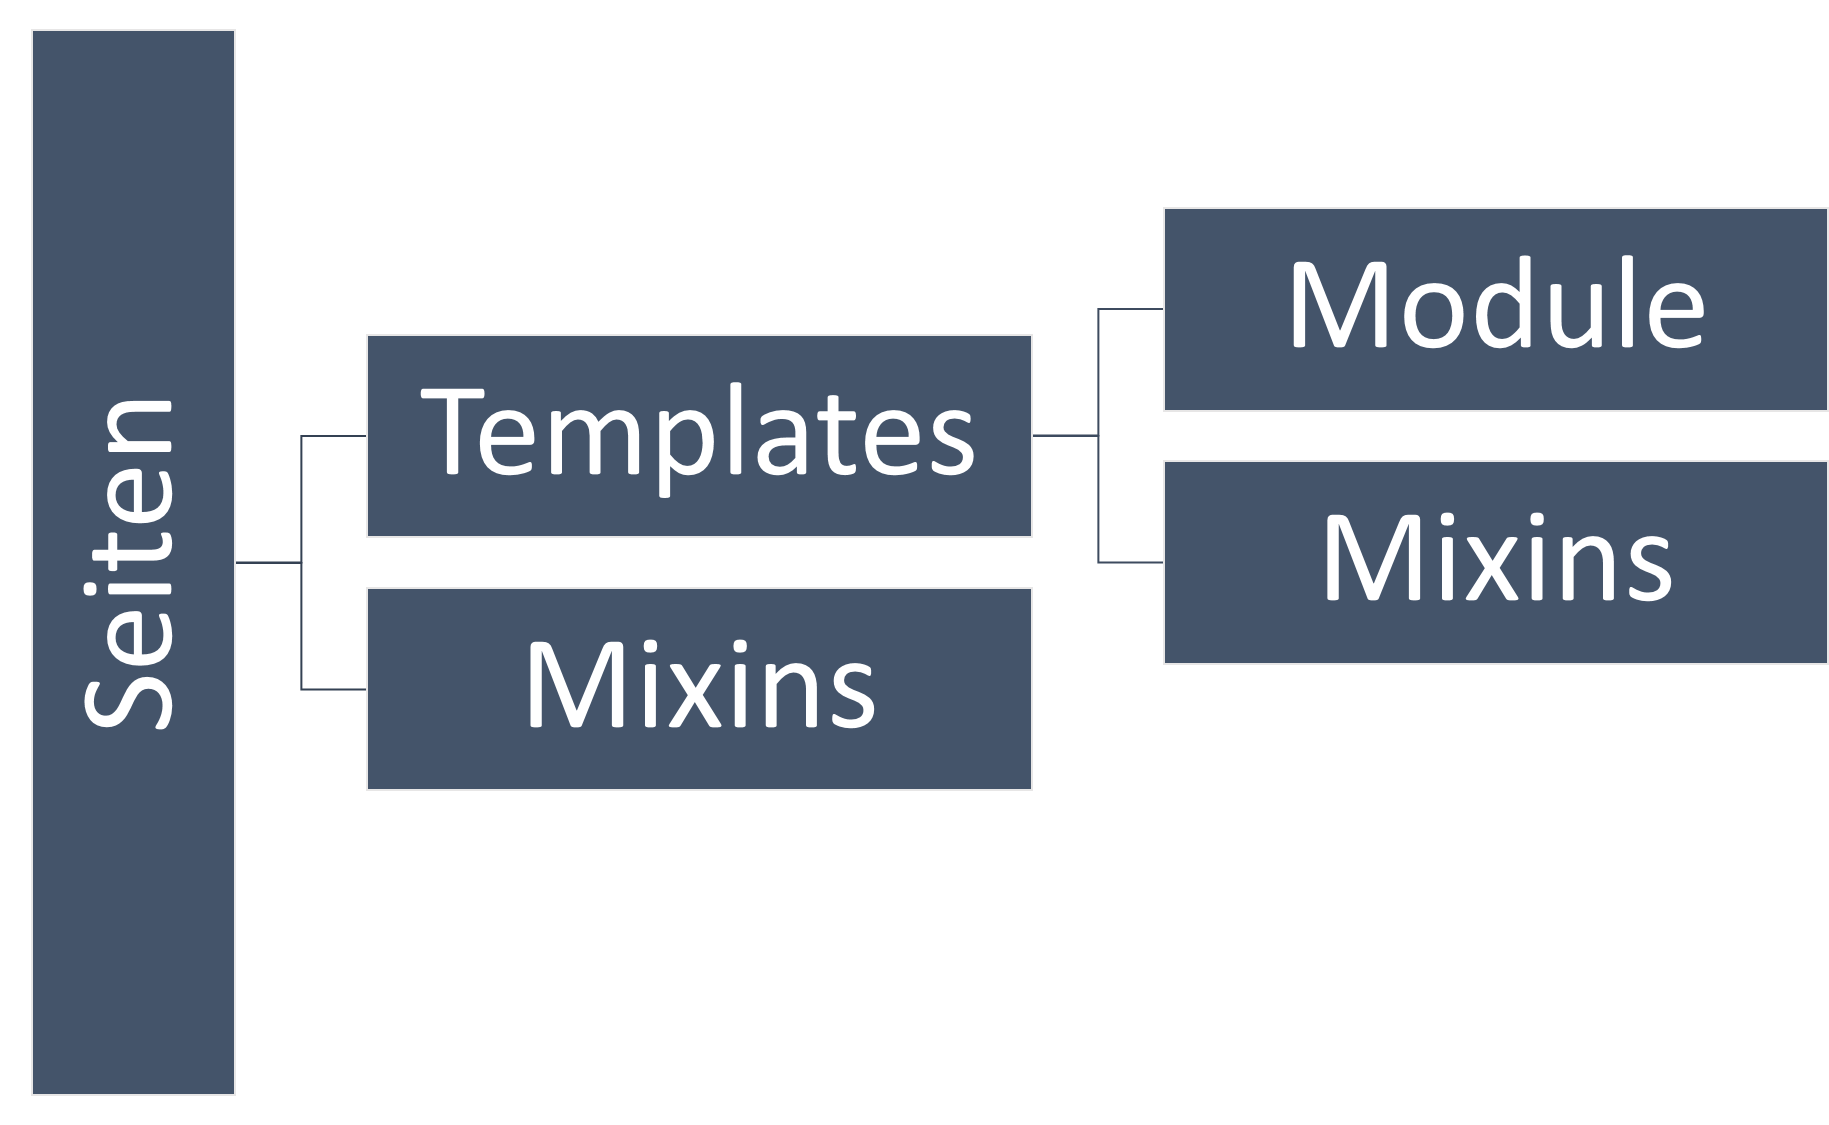
\includegraphics[width=\textwidth]{./img/pre_system.png}
	\caption{Hierarchische Darstellung des Templating-Systems.}
	\label{pre:system}
\end{figure}